\documentclass{article}
\usepackage[utf8]{inputenc}
\usepackage{amsmath, scalefnt}
\usepackage{amsthm}
\usepackage{amssymb}
\usepackage{amsfonts}
%\usepackage{wrapfig}
%\usepackage{geometry}
%\geometry{ hmargin=2.8cm, vmargin=3cm }
\usepackage{graphicx}
%\usepackage{amsmath}
%\usepackage{mathdots}
\input def_algolight.tex

\theoremstyle{plain}% default
\newtheorem{thm}{Théorème}
\newtheorem{conj}{Conjecture}
\newtheorem{lem}{Lemme}
\newtheorem{prop}{Proposition}
\newtheorem{cor}{Corollaire}

\theoremstyle{definition}
\newtheorem{defn}{Définition}
\newtheorem{exmp}{Example}


\theoremstyle{remark}
\newtheorem*{rem}{Remarque}
\newtheorem*{note}{Note}
\newtheorem*{case}{Case}

\def\R{\mathbb{R}}
\newcommand{\vecb}[1]{\pmb{#1}}
\newcommand{\VECAXPY}{\textsc{VecAxpy}}

\newcommand{\cA}{\mathcal{A}}
\newcommand{\cM}{\mathcal{M}}
\newcommand{\cS}{\mathcal{S}}
\newcommand{\cR}{\mathcal{R}}
\newcommand{\cU}{\mathcal{U}}
\newcommand{\bcA}{\boldsymbol{\cA}}
\newcommand{\bcS}{\boldsymbol{\cS}}
\newcommand{\bvpi}{\boldsymbol{\varpi}}

\newcommand{\wcM}{\widetilde\cM}
\newcommand{\wcU}{\widetilde\cU}

\newcommand{\VT}{\Vert T_n \Vert}
\newcommand{\VcM}{\Vert \cM_n \Vert}
\newcommand{\VwcM}{\Vert \widetilde\cM_n \Vert}
\newcommand{\VcU}{\Vert \cU_n \Vert}
\newcommand{\VwcU}{\Vert \widetilde\cU_n \Vert}
\newcommand{\bi}{\boldsymbol{\infty}}
\newcommand{\bpi}{\boldsymbol{\pi}}
\newcommand{\bmu}{\boldsymbol{\mu}}
\newcommand{\N}{\mathbb{N}}
\newcommand{\Z}{\mathbb{Z}}
\newcommand{\C}{\mathbb{C}}
\newcommand{\ov}{\overline}
\newcommand{\wh}{\widehat}
\newcommand{\sn}{\sqrt{n}}


\begin{document}


%% Title, authors and addresses

\title{A polynomial solver based on numerical linear algebra : practical implementation and numerical experiments.}
\author{Jean-Paul Cardinal}



\begin{abstract}
%~ Nous proposons un algorithme de calcul
%~ numérique des racines d'un système polynômial zéro-dimensionnel basé sur les matrices de Bézout.
%~ Cet algorithme est entièrement basé sur des procédures l'algèbre linéaire numérique. Une implémentation en python en est fournie en annexe.
\end{abstract}


\section{Introduction}


\section{Cas univariable}
\label{univariable}

Rappelons quelques faits connus sur les polynômes à une variable.\\
Soit $f(x) = a_0x^d + \dots + a_{d-1}x + a_d$ un polynôme de la variable complexe $x$. Notons $<f(x)>$ l'idéal engendré par $f(x)$ dans l'anneau $\C[x]$ et $A_x = \C[x]/<f(x)>$  son algèbre quotient; de même nous noterons $A_y = \C[y]/<f(y)>$. Dorénavant $x$ désignera indifféremment la variable $x$, sa projection sur le quotient $A_x$ ou l'endomorphisme de multiplication par $x$ dans $A_x$. Une base du $\C$-espace vectoriel $A_x$ est de dimension $d$ dont une base, appelée {\bf base des monômes}, est $\bold{x} = (1, x,\cdots, x^{d-1})$ famille d'éléments élément de $A_x$.

\subsection{Matrices des opérateurs de multiplication dans $A_x$}
L'opérateur de multiplication
$x = \left\vert
\begin{array}{c}
A \mapsto A \\
h \mapsto xh
\end{array}
\right.$ est un endomorphisme et se représente donc dans la base des monômes par
une matrice $X$ de taille $d$, appelée {\bf la matrice compagnon}
\begin{equation}
\label{compan}
X =
\begin{bmatrix}
	0 & \cdots & 0 & -a_d/a_0 \\
	1 & 0 & \cdots & -a_{d-1}/a_0 \\
	\vdots  & \ddots  & \ddots & \vdots  \\
	0 & \cdots & 1 & -a_1/a_0
\end{bmatrix}
\end{equation}

\begin{prop}
\label{compan2roots}
La matrice compagnon admet $f$ comme polynôme caractéristique et comme polynôme minimal, c'est-à-dire que $f(X) = 0$. De plus les racines du polynôme $f$ sont les valeurs propres de $X$, comptées avec les mêmes multiplicités.
\end{prop}

\begin{rem}
La proposition précédente fournit une méthode effective de calcul numérique des racines de $f$. En effet, $X$ est une matrice de Hessenberg, à laquelle on peut appliquer des techniques performantes de calcul de valeurs propres, comme la méthode du QR. Nous appliquerons aussi ces techniques dans le cas d'un système multivariable.
\end{rem}
Plus généralement, pour un élément $g\in A_x$, l'opérateur de multiplication
$g = \left\vert
\begin{array}{c}
A \mapsto A \\
h \mapsto gh
\end{array}
\right.$
est un endomorphisme, qui se représente dans la base des monômes par une matrice que nous appelerons encore {\bf matrice compagnon de $g$} et qui se calcule à partir de $X$ très facilement. Considérons par exemple $g = x^2$. L'opérateur de multiplication par $x^2$ n'est autre que l'opérateur de multiplication par $x$, lui-même élevé au carré. Sa matrice est donc $X^2$. Plus généralement, nous avons
\begin{prop}
la matrice compagnon de $g$ est $g(X)$.
\end{prop}

\begin{rem}
Il faut noter que si $g_1, g_2$ sont deux représentants de $g$ on a $g_1(X) = g_2(X)$, ce qui définit $g(X)$ sans ambiguité, indépendamment du représentant de $g$ dans $A_x$.
\end{rem}

\subsection{Polynômes et matrices de Bezout}
\begin{defn}
\label{def_bez}
Introduisons une nouvelle variable $y$.
%et une famille $\bold{y} = (1, y, \cdots, y^{d-1})$, d'éléments de $A_y$.
Pour tout polynôme $g$, on définit le {\bf polynôme de Bezout $\delta(g)$} et la {\bf matrice de Bezout $B(g) = [b_{\alpha\beta}]$}  par les formules
\begin{equation}
\delta(g) = \dfrac{f(x)g(y)-f(y)g(x)}{x-y} = \sum_{\alpha,\beta = 0, \cdots, m-1} b_{\alpha\beta} x^\alpha y^\beta
\end{equation}
où $m$ désigne n'importe quel entier supérieur ou égal au maximum des degrés de $f$ et $g$.
\end{defn}

\begin{rem}
Le polynôme et la matrice de Bezout sont liés par l'égalité matricielle
\begin{equation}
	\delta(g) = \bold{x} B(g) \bold{y}^T
\end{equation}
où $\bold{x} = (1, x,\cdots, x^{m-1})$ et $\bold{y} = (1, y,\cdots, y^{m-1})$ sont des vecteurs de monômes de $\C[x]$ et $\C[y]$. (Attention, on emploie encore ici la notation ${\bold x}$ pour un vecteur de $\C[x]^m$, notation qui était utilisée précédemment pour désigner la base des monômes ${\bold x}$ mais en pratique cette confusion n'est pas gênante).
Considérons maintenat les produits vecteur-matrice $\bold{x}B(1)$ et $\bold{x}B(g)$. Ces deux familles sont constituées des colonnes de $B(1)$, resp. $B(g)$, vues comme des polynômes en $x$ exprimés dans la base des monômes. On peut aussi voir $\bold{x}B(1)$, resp. $\bold{x}B(g)$, comme la famille des coefficients de $\delta(1)$, resp. $\delta(g)$, considéré comme un polynôme en $y$ à coefficients dans $\C[x]$.
\end{rem}

\begin{prop}
\label{relations_prop}
Soit $g$ un polynôme de $\C[x]$, et $m$ le maximum des degrés de $f$ et $g$. Si on écrit $B(1)$ et $B(g)$ dans le même système d'indice $\bold{x} = (1, x,\cdots, x^{m-1})$ et $\bold{y} = (1, y,\cdots, y^{m-1})$, alors
\begin{equation}
\label{relations}
	\bold{x}B(1)g = \bold{x}B(g)
\end{equation}
\end{prop}
\begin{proof}
Ecrivons
\begin{align} \nonumber
	\delta(g) = g(x)\dfrac{f(x)-f(y)}{x-y} - f(x)\dfrac{g(x)-g(y)}{x-y} \\ \nonumber
	\delta(g) = g(x)\delta(1) - f(x)\dfrac{g(x)-g(y)}{x-y}
\end{align}
Regardons cette dernière égalité comme une égalité entre polynômes en la variable $y$, à coefficients dans $\C[x]$. Si $h\in \C[x][y]$ et $\beta\in\N$ notons $h_\beta$ le coefficient de $y^\beta$ dans $h$. On a alors
$$\delta(g)_\beta = g(x)\delta(1)_\beta - f(x)(\dfrac{g(x)-g(y)}{x-y})_\beta $$
qui est une égalité entre éléments de $\C[x]$. En projetant sur $A_x$ on a
$\delta(g)_\beta = g(x)\delta(1)_\beta$
et comme ceci est vrai pour tout $\beta\in\N$, on obtient bien la relation \ref{relations}.
\end{proof}
\begin{rem}
En disant la  proposition autrement, chaque colonne de $B(1)$ donne, lorsqu'elle est multipliée par $g$ modulo $A_x$, la colonne de même indice de $B(g)$.
\end{rem}
\begin{exmp}
Pour $f = x^2 - 3x + 2$, et $g = x^3$ on a
$$
\begin{array}{c|ccc}
\delta(1) & 1 & y & y^2\\
\hline
1 & -3 & 1 & 0\\
x & 1 & 0 & 0\\
x^2 & 0 & 0 & 0
\end{array}
\hspace{1cm}
\begin{array}{c|ccc}
\delta(x^3) & 1 & y & y^2\\
\hline
1 & 0 & 0 & -2\\
x & 0 & -2 & 3\\
x^2 & -2 & 3 & -1
\end{array}
$$
La proposition \ref{relations_prop} dit que, modulo $A_x$,
\begin{align} \nonumber
	(-3 + x)x^3 &= -2x^2 \\ \nonumber
	(1)x^3 &= -2x + 3x^2 \\ \nonumber
	(0)x^3 &= -2 + 3x - x^2
\end{align}
ce qui se vérifie facilement.
\end{exmp}

\begin{rem}
En considérant les lignes de $B(1), B(x)$ à la place des colonnes on aboutirait à une formule écrite en la variable $y$, identique à la formule \ref{relations} car les matrices de Bezout sont ici symétriques, mais ce ne sera plus le cas en plusieurs variables.
\end{rem}

%\begin{rem}
%Les relations \ref{relations} sont d'un extrême importance pour nous et seront utilisées dans la construction du quotient dans le cas multivariable. Pour le dire à nouveau,, phénomène qui se traduit matriciellement par la formule de Barnett.
%\end{rem}

\subsection{Lien entre matrices de Bezout et matrices compagnon}
\label{Bar}
Particulièrement importantes sont les matrices de Bezout définies par $B(1)$ et $B(x)$
\begin{equation}
	\begin{array}{c|cccc}
		\delta(1) & 1 & y & \dots & y^{d-1} \\
		\hline
		1 & a_{d-1} & \ldots & \dots & a_0 \\
		x & a_{d-2} & \dots & a_0 & 0 \\
		\vdots & \vdots & \vdots & \vdots & \vdots \\
		x_{d-1} & a_0 & 0 & \ldots & 0 \\
	\end{array}
	\hspace{1.5cm}
	\begin{array}{c|cccc}
		\delta(x) & 1 & y & \dots & y^{d-1} \\
		\hline
		1 & -a_{d} & 0 & \dots & 0 \\
		x & 0 & a_{d-2} & \ldots & a_0 \\
		\vdots & \vdots & \vdots & \vdots & \vdots \\
		x_{d-1} & 0 & a_0 & \ldots & 0 \\
	\end{array}
\end{equation}
en effet nous avons le lien suivant entre matrice de Bezout et la matrice compagnon
\begin{prop}
\label{Barnett}
La matrice compagnon $X$ peut se calculer grâce à la {\bf formule de Barnett}
\cite{Barnett}
\begin{equation}
	B(x)B(1)^{-1} = X
\end{equation}
\end{prop}
\begin{proof}
Définissons deux nouvelles familles dans $A_x$ par
\begin{equation}
	\begin{array}{lll}
		\bold{x}B(1) & = & (a_{d-1} + a_{d-2}x + \cdots + a_0x^{d-1}, \cdots, a_1 + a_0x,  a_0).\\
		\bold{x}B(x) & = & (-a_d, a_{d-2}x + \cdots + a_0x^{d-1}, \cdots, a_0x)
	\end{array}
\end{equation}
et posons $\hat{\bold{x}} = \bold{x}B(1)$.
$B(1)$ étant inversible, la famille $\hat{\bold{x}}$ est une base de $A_x$ appellée {\bf base de Horner}.
D'après la proposition \ref{relations_prop} on a $\hat{\bold{x}}x = \bold{x}B(1)$. Par construction, les familles $\hat{\bold{x}}$ et $\hat{\bold{x}}x$ s'expriment dans la base $\bold{x}$ (des monômes) respectivement par les matrices $B(1)$ et $B(x)$. La famille $\hat{\bold{x}}x$ s'exprime donc dans la base $\hat{\bold{x}}$ (de Horner) par la matrice $B(1)^{-1}B(x)$ ce qui veut dire que l'endomorphisme
$x = \left\vert
\begin{array}{c}
A \mapsto A \\
h \mapsto xh
\end{array}
\right.$ a pour matrice $B(1)^{-1}B(x)$ dans la base $\hat{\bold{x}}$
et pour matrice $B(1)(B(1)^{-1}B(x))B(1)^{-1} = B(x)B(1)^{-1}$ dans la base $\bold{x}$.
\end{proof}



\subsection{Formule de Barnett généralisée}
\label{Bar_gen}
La formule de Barnett a été écrite en considérant les matrices de Bezout des polynômes $1$ et $x$.
Si on considère un polynôme quelconque $g$ de $\C[x]$ et $B(g)$ sa matrice de Bezout il serait naturel d'avoir entre les matrices de Bezout $B(1)$ et $B(g)$ la relation suivante, que nous appellerons {\bf formule de Barnett généralisée}
\begin{equation}
	\label{BG}
	B(g)B(1)^{-1} = g(X)
\end{equation}
On montre facilement la formule \ref{BG} lorsque le degré de g est inférieur ou égal à $d$, c'est-à-dire lorsque $B(1)$ et $B(g)$ sont de même taille. Par exemple pour $f = x^2 - 3x + 2$, $d = 2$, on a
$$
\begin{array}{c|cc}
	\delta(1) & 1 & y \\
	\hline
	1 & -3 & 1 \\
	x & 1 & 0
\end{array}
\hspace{1cm}
\begin{array}{c|cc}
	\delta(x) & 1 & y \\
	\hline
	1 & -2 & 1 \\
	x & 1 & 0
\end{array}
\hspace{1cm}
\begin{array}{c|cc}
	\delta(x^2) & 1 & y \\
	\hline
	1 & 0 & -2 \\
	x & -2 & 3
\end{array}
$$
\begin{equation}
	B(x)B(1)^{-1} =
	\begin{bmatrix}
		0 & -2 \\
		1 & 3
	\end{bmatrix}
	= X
	\hspace{1cm}
	B(x^2)B(1)^{-1} =
	\begin{bmatrix}
		-3 & -6 \\
		2 & 7
	\end{bmatrix}
	= X^2
\end{equation}
ce qui confirme bien la formule \ref{BG}.
Si par contre le degré de $g$ est supérieur à $d$, alors $B(g)$ et $B(1)$ ne sont plus de la même taille et une opération telle que $B(g)B(1)^{-1}$ n'a plus de sens. Une première idée est de réécrire les deux matrices de Bezout dans le même système d'indices, à savoir
$\bold{x} = (1, x,\cdots, x^{m-1})$ et $\bold{y} = (1, y,\cdots, y^{m-1})$, $m$ étant le degré de $g$. Par exemple en choisissant $f$ comme ci-dessus et $g = x^3$ on aurait
$$
\begin{array}{c|ccc}
\delta(1) & 1 & y & y^2\\
\hline
1 & -3 & 1 & 0\\
x & 1 & 0 & 0\\
x^2 & 0 & 0 & 0
\end{array}
\hspace{1cm}
\begin{array}{c|ccc}
\delta(x^3) & 1 & y & y^2\\
\hline
1 & 0 & 0 & -2\\
x & 0 & -2 & 3\\
x^2 & -2 & 3 & -1
\end{array}
$$
mais alors $B(1)$ n'est plus inversible. Nous allons cependant montrer, grâce aux relations \ref{relations}, que si {\bf on projette les deux polynômes de Bezout sur le quotient $A_x$} alors les matrices $B(g)$ et $B(1)$ sont redimensionnées à la même taille, $B(1)$ est inversible et la formule \ref{BG} s'applique. Illustrons le procédé sur l'exemple ci-dessus.
Puisque $B(1)$ n'est pas inversible, on peut trouver une combinaison linéaire de colonnes qui s'annule, ici c'est la troisième colonne qui est nulle. En la multipliant par $x^3$, et en appliquant les  relations \ref{relations}, on obtient que la troisième colonne de $B(x^3)$ est aussi nulle. Mais cette colonne vaut $-2 + 3x - x^2$ ce qui entraine que, dans le quotient, $-2 + 3x - x^2 = 0$ (ce n'est pas une surprise car ce dernier polynôme n'est autre que $-f$; ceci est dû au fait que l'exemple choisi est particulièrement simple, mais nous verrons dans le cas multidimensionnel que les relations nulles dans le quotient ainsi générées sont loin d'être triviales).
En vue d'automatiser les calculs, traduisons le procédé précédent en termes d'algèbre matricielle.
Toujours sur le même exemple
\begin{align} \nonumber %%%%%%%%%%%%%%
	\delta(x^3) &=
	\begin{bmatrix}
			1 & x & x^2
	\end{bmatrix}
	\begin{bmatrix}
		0 & 0 & -2 \\
		0 & -2 & 3 \\
		-2 & 3 & -1
	\end{bmatrix}
	\begin{bmatrix}
		1 \\
		y \\
		y^2
	\end{bmatrix} \\ \nonumber %%%%%%%%%%%%%%
	\delta(x^3) &=
	\begin{bmatrix}
		1 & x & x^2
	\end{bmatrix}
	\begin{bmatrix}
		1 & 0 & 2 \\
		0 & 1 & -3 \\
		0 & 0 & 1
	\end{bmatrix}
	\begin{bmatrix}
		1 & 0 & -2 \\
		0 & 1 & 3 \\
		0 & 0 & 1
	\end{bmatrix}
	\begin{bmatrix}
		0 & 0 & -2 \\
		0 & -2 & 3 \\
		-2 & 3 & -1
	\end{bmatrix}
	\begin{bmatrix}
		1 \\
		y \\
		y^2
	\end{bmatrix} \\ \nonumber %%%%%%%%%%%%%%%
	\delta(x^3) &=
	\begin{bmatrix}
			1 & x & 2 - 3x + x^2
	\end{bmatrix}
	\begin{bmatrix}
		4 & -6 & 0 \\
		-6 & 7 & 0 \\
		-2 & 3 & -1
	\end{bmatrix}
	\begin{bmatrix}
		1 \\
		y \\
		y^2
	\end{bmatrix} \\ \nonumber %%%%%%%%%%%%%%
\end{align}
En résumé nous multiplions le vecteur d'indices
$\begin{bmatrix}
	1 & x & x^2
\end{bmatrix}$ à droite par la transformation de Gauss
$P =
\begin{bmatrix}
	1 & 0 & 2 \\
	0 & 1 & -3 \\
	0 & 0 & 1
\end{bmatrix}$, les deux matrices de Bezout $B(1)$ et $B(g)$ à gauche par
$P^{-1} =
\begin{bmatrix}
	1 & 0 & -2 \\
	0 & 1 & 3 \\
	0 & 0 & 1
\end{bmatrix}$. Les polynômes de Bezout, écrits sous la forme de tableaux, deviennent alors
$$
\begin{array}{c|ccc}
	\delta(1) & 1 & y & y^2\\
	\hline
	1 & -3 & 1 & 0\\
	x & 1 & 0 & 0\\
	2 - 3x + x^2 & 0 & 0 & 0
\end{array}
\hspace{1cm}
\begin{array}{c|ccc}
	\delta(x^3) & 1 & y & y^2\\
	\hline
	1 & 4 & -6 & 0 \\
	x & -6 & 7 & 0 \\
	2 - 3x + x^2 & -2 & 3 & -1
\end{array}
$$
Ce que disent les relations \ref{relations} c'est que la troisième colonne de $B(x^3)$ est nulle dans le quotient $A_x$, c'est à-dire $-2 + 3x - x^2 = 0$, (on reconnait l'égalité $-f = 0$). On a donc

$$
\delta(1) = \begin{bmatrix}
	1 & x
\end{bmatrix}
\begin{bmatrix}
	-3 & 1 \\
	1 & 0
\end{bmatrix}
\begin{bmatrix}
	1 \\
	y
\end{bmatrix},
\hspace{1cm}
\delta(x^3) = \begin{bmatrix}
	1 & x
\end{bmatrix}
\begin{bmatrix}
	4 & -6 \\
	-6 & 7
\end{bmatrix}
\begin{bmatrix}
	1 \\
	y
\end{bmatrix} - (2 - 3x + x^2)(2 - 3y + y^2)
$$


puis, en projetant $\delta(1), \delta(g)$ sur $A_x \otimes A_y$
$$
\begin{array}{c|cc}
	\delta(1) & 1 & y \\
	\hline
	1 & -3 & 1 \\
	x & 1 & 0
\end{array}
\hspace{1cm}
\begin{array}{c|cc}
	\delta(x^3) & 1 & y \\
	\hline
	1 & 4 & -6  \\
	x & -6 & 7
\end{array}
$$

Nous avons bien obtenu des matrices de Bezout de même taille, avec $B(1)$ inversible. Formons alors le quotient
\begin{equation}
	B(x^3)B(1)^{-1} =
	\begin{bmatrix}
		-6 & -14 \\
		7 & 15
	\end{bmatrix}
	= X^3
\end{equation}
ce qui est bien conforme à la formule de Barnett généralisée.

\begin{rem}
On peut remplacer la matrice de Gauss par toute matrice permettant de transformer une colonne donnée en une colonne possédant un seul élément non nul, comme par exemple une matrice orthogonale de Householder. C'est le choix qui sera fait dans l'implémentation en Octave proposée en annexe.

\end{rem}

%Nous voyons donc que la matrice compagnon peut être calculée à partir de matrices de Bezout,
%phénomène qui n'est pas, en une variable, particulièrement intéressant, mais qui sera, dans le cas multivariable, pleinement exploité pour le calcul des matrices compagnon et de la structure de l'algèbre quotient $A$.


\section{Cas multivariable}
Dans le cas univariable, examiné à la section précédente, la structure de $A_x$ se compose de deux éléments : d'une part une base, en l'occurence la base des monômes, d'autre part la matrice compagnon, exprimant l'endomorphisme de multiplication par $x$ dans la base. Ces deux éléments peuvent être obtenus soit directement par lecture des coefficients de $f$, soit à partir des matrices de Bezout $B(1), B(x)$. \\
Dans le le cas multivariable, que nous allons développer dans cette section, ni une base ni les matrices compagnon
(matrices des opérateurs
$x_j = \left\vert
\begin{array}{c}
A \mapsto A \\
h \mapsto x_jh
\end{array}
\right.$ dans la base) ne sont visibles directement sur les coefficients des polynômes de départ. En revanche nous allons montrer comment construire des matrices de Bezout $B(1), B(x_1), \cdots, B(x_n)$ à partir desquelles on peut obtenir une base et les matrices compagnon $X_j$ associées à la base obtenue. Commençons par fixer le cadre de travail.
On considère $n$ polynômes $f_1,\cdots, f_n$ en les variables complexes $x_1,\cdots, x_n$. Notons :
\begin{itemize}
\item $\C[x] = \C[x_1,\cdots, x_n]$ l'anneau des polynômes en les variables $x = x_1,\cdots, x_n$
\item $<f> = <f_1,\cdots, f_n>$ l'idéal qu'ils génèrent,
\item $V(f) = \{x \in \C^n : f(x) = 0\}$ la variété associée à $<f>$
\item $A_x = \C[x]/<f>$ l'algèbre quotient
\end{itemize}
Nous supposerons dorénavant que l'idéal $<f>$ est {\bf zéro-dimensionel},
c'est-à-dire que $V(I)$ est fini ou, de façon équivalente  (see \cite{clo} p..), que {\bf $A_x$ est de dimension finie} en tant qu'espace vectoriel sur $\C$. Ceci est bien sûr toujours le cas lorsque $n = 1$.

\subsection{Construction des polynômes et des matrices de Bezout dans le cas multivariable}

\subsubsection{Extension de la définition \ref{def_bez} au cas multivariable.}
\label{def_bez_multi}

\begin{defn}
Soit $x^\gamma = x_1^{\gamma_1}\cdots x_n^{\gamma_n} \in \C[x]$ un monôme.
Introduisons un nouveau jeu de variables $y = y_1,\cdots, y_n$ et considérons, pour tous $i, j = 1\cdots n$, le rapport
\begin{equation}
\label{finite_diff}
\delta_{i,j}(x^\gamma) = \dfrac{y_j^{\gamma_j}f_i(y_1,\cdots, y_{j-1},x_j,\cdots,x_n) - x_j^{\gamma_j}f_i(y_1,\cdots,y_j,x_{j+1},\cdots,x_n)}{x_j - y_j}
\end{equation}
qui est un polynôme en les variables $x, y$. Nous obtenons une matrice de différences finies $\Delta(x^\gamma) = (\delta_{ij}(x^\gamma))_{ij}$, qui est à la matrice jacobienne ce que le taux d'accroissement est à la dérivée.
Le {\bf polynôme de Bezout} du monôme $x^\gamma$ est par définition
\begin{equation}
	\delta(x^\gamma) = det(\Delta(x^\gamma))
\end{equation}
qui est un élément de $\C[x, y]$. Pour un polynôme général $g = \sum_\gamma g_\gamma x^\gamma \in \C[x]$, on étend la définition précédente par linéarité $\delta(g) = \sum_\gamma g_\gamma \delta(x^\gamma)$.
En développant $\delta(g) = \sum_{\alpha,\beta} b_{\alpha\beta} x^\alpha y^\beta$ comme une somme de monômes de $\C[x, y]$, et en notant $\bold{x}$ et $\bold{y}$ les familles de tous les monômes en $x$ et $y$ apparaissant dans ce développement, nous définissons la {\bf matrice de Bezout} $B(g) = [b_{\alpha\beta}]$, c'est à dire que l'on a
\begin{equation}
	\delta(g) = \bold{x} B(g) \bold{y}^T
\end{equation}
\end{defn}

\begin{exmp}
\label{ex_bez_multi}
Fixons $n = 2$ et considérons $f_1 = x_1^2 + x_1x_2^2 - 1, f_2 = x_1^2x_2 + x_1$.
Nous allons calculer les matrices de Bezout $B(1), B(x_1), B(x_2)$,  qui vont servir à la construction des matrices compagnon $X_1, X_2$, comme nous le verrons plus loin. Pour commencer, calculons à partir des formules (\ref{finite_diff})
\begin{align}
\Delta(1) &=
\begin{pmatrix}
x_1 + x_2^2 + y_1 & x_2y_1 + y_1y_2 \\
1 + x_1x_2 + x_2y_1 & y_1^2
\end{pmatrix} \nonumber  \\
\Delta(x_1) &=
\begin{pmatrix}
1 + x_1y_1 & x_2y_1 + y_1y_2 \\
1 + x_1x_2 + x_2y_1 & y_1^2
\end{pmatrix} \nonumber  \\
\Delta(x_2) &=
\begin{pmatrix}
x_1 + x_2^2 + y_1 & 1 - y_1^2 + x_2y_1y_2 \\
1 + x_1x_2 + x_2y_1  & -y_1
\end{pmatrix} \nonumber
\end{align}
dont le déterminant fournit les polynômes de Bezout
\begin{align}
\delta(1) &= -x_2y_1 - x_1x_2^2y_1 + x_1y_1^2 + y_1^3 - y_1y_2 - x_1x_2y_1y_2 - x_2y_1^2y_2 \nonumber \\
\delta(x_1) &=  y_1^2 - x_1x_2^2y_1^2 + x_1y_1^3 - x_1x_2y_1^2y_2 \nonumber \\
\delta(x_2) &= -1 - x_1x_2 - x_1y_1 -x_2y_1 - x_2^2y_1 + x_1x_2y_1^2 + x_2y_1^3 - x_2y_1y_2 - x_1x_2^2y_1y_2 - x_2^2y_1^2y_2\nonumber
\end{align}
Les familles de mônomes apparaissant dans ces polynômes sont
$\bold{x} = (1, x_2, x_2^2, x_1, x_1x_2, x_1x_2^2)$ et $\bold{y} = (1, y_1, y_1y_2, y_1^2, y_1^2y_2, y_1^3)$.
Les polynomes de Bezout s'écrivent sous forme de tableaux\\

\resizebox{\linewidth}{!}{$
\begin{array}{c|cccccc}
	\delta(1) & 1 & y_1 & y_1y_2 & y_1^2 & y_1^2y_2 & y_1^3 \\
	\hline
	1 &  &  & -1 &  &  & 1\\
	x_2 &  & -1 &  &  & -1 & \\
	x_2^2 &  &  &  &  &  & \\
	x_1 &  &  &  & 1 &  & \\
	x_1x_2 &  &  & -1 &  &  & \\
	x_1x_2^2 &  & -1 &  &  &  &
\end{array}
\hspace{0.2cm}
\begin{array}{c|cccccc}
	\delta(x_1) & 1 & y_1 & y_1y_2 & y_1^2 & y_1^2y_2 & y_1^3 \\
	\hline
	1 &  &  &  & 1 &  & \\
	x_2 &  &  &  &  &  & \\
	x_2^2 &  &  &  &  &  & \\
	x_1 &  &  &  &  &  & 1\\
	x_1x_2 &  &  &  &  & -1 & \\
	x_1x_2^2 &  &  &  & -1 &  &
\end{array}
\hspace{0.2cm}
\begin{array}{c|cccccc}
	\delta(x_2) & 1 & y_1 & y_1y_2 & y_1^2 & y_1^2y_2 & y_1^3 \\
	\hline
	1 & -1 &  &  &  &  & \\
	x_2 &  & -1 & -1 &  &  & 1\\
	x_2^2 &  & -1 &  &  & -1 & \\
	x_1 &  & -1 &  &  &  & \\
	x_1x_2 & -1 &  &  & 1 &  & \\
	x_1x_2^2 &  &  & -1 &  &  &
\end{array}
$}
\end{exmp}
\begin{rem}
Ici, contrairement à la situation en une variable, les listes $\bold{x}$ et $\bold{y}$ ne sont pas des bases de $A$. Nous verrons plus loin qu'elles sont cependant génératrices et comment on peut en extraire des bases.
\end{rem}
\subsubsection{Calcul effectif des matrices de Bezout}
Dans l'exemple précédent, les polynômes de Bezout s'obtiennent en calculant le déterminant des matrices $\Delta(1), \Delta(x_1), \Delta(x_2)$, qui sont de taille $2$ et dont les coefficients sont des polynômes en $x_1, x_2$. Si $n$ ou les degrés des polynômes$f_i$ augmentent ce calcul peut devenir difficile car les coefficients des matrices $\Delta(x_j)$ ne sont pas numériques et on ne peut donc pas appliquer la méthode du pivot de Gauss. Voici un moyen de contourner cette difficulté. D'une façon générale, pour calculer le déterminant d'une matrice à coefficients polynômiaux, comme $\Delta(x^\gamma)$, on peut procéder par évaluation-interpolation :

\begin{itemize}
\item estimation à priori de l'ensemble des monômes qui vont apparaitre dans le résultat $\delta(x^\gamma)$
\item évaluation de $\Delta(x^\gamma)$ sur un ensemble adéquat de multi-points de Fourier $u = (u_1,\cdots, u_n, v_1,\cdots, v_n) ) \in U\times V$
\item pour chaque point $(u, v) \in U\times V$ calcul du déterminant numérique de $\Delta(x^\gamma)(u, v)$ par la méthode du pivot de Gauss.
\item interpolation de l'ensemble des valeurs obtenues par le polynôme cherché $\delta(x^\gamma)$.
\end{itemize}

\begin{algorithm}[H]
\caption{Function \texttt{FourierBezout} \ renvoie $B_j = B(x_j)$  la matrice de Bezout construite à partir d'un système polynômial $f$ et d'une variable $x_j$.}\label{algo:01}
%\begin{minipage}{14.cm}
\textbf{Input\ }
  \begin{tabular}[t]{lcl}
    $\vecb{f}$  & : &  système $(f_1, \cdots, f_n)$ de $n$ polynômes de $\C^n$, de multi-degré $(d_1, \cdots, d_n)$,\\
     $\vecb{j}$ & : & un entier compris entre $0$ et $n$.
  \end{tabular}\\
\textbf{Output\ }
  \begin{tabular}[t]{lcl}
      $\vecb{B_j}$  & : & la matrice de Bezout $B(x_j)$ associée à la variable $x_j$.
  \end{tabular}
%\end{minipage}
\begin{algorithmic}
\Function{$B_j \gets$ \texttt{FourierBezout}}{ $f$ }
	\State Création des points de Fourier $U = \prod_{j=1..n} F_{jd_j}$ et $V = \prod_{j=1..n} F_{(n-j+1)d_j}$
	\State $C \gets \texttt{zeros}(D, D)$
	\For{$(u, v) \in U\times V$}
   		\For{$(i, j) \gets 1..n$}
      		\State $m(i, j) \gets \Delta_j f_i(u, v)$
   		\EndFor
		\State $C(u, v) \gets \texttt{det}(m)$
	\EndFor
\EndFunction
\end{algorithmic}
\end{algorithm}

\begin{rem}
Les polynômes de Bezout les plus généraux s'obtiennent à partir de différents $\delta(x^\gamma)$ par linéarité mais en pratique, dans cet article, seuls les polynômes $\delta(1),\delta(x_1),\cdots,\delta(x_n)$ seront considérés.
\end{rem}

\subsection{Formules de Barnett et structure de l'algèbre quotient.}

Rappelons que dans notre hypothèse où l'idéal est zéro-dimensionel, la dimension de l'algèbre quotient $A = \C[\bold{x}]/<f>$ est finie, ce qui assure l'existence d'une base et de matrices compagnon $X_1,\cdots, X_n$ (matrices des opérateurs de multiplication par les variables dans la base considérée). Nous allons montrer que le procédé mis en oeuvre dans la section \ref{Bar_gen}, consistant en manipulations sur les colonnes des matrices de Bezout $B_0, \cdots, B_n $, permettra de construire une base de $A_x$ ainsi que les matrices compagnons associées.\\
Rappelons tout d'abord un certain nombre de propriétés algébriques du polynôme $\delta(1)$ et des matrices de Bezout $B_j$.

\subsubsection{Propriétés algébriques du polynôme $\delta(1)$ et de la matrice $B_0$}
Les propriétés qui suivent sont de nature algébrique et seront données sans démonstration. Le lecteur intéressé pourra consulter les détails dans \cite{jpc, CM}. Comme dans la proposition \ref{Barnett}, définissons de nouvelles familles dans $A_x$ par
\begin{equation}
		\hat{\bold{x}}_j  =  \bold{x}B_j, \quad j=0\cdots n
\end{equation}

\begin{exmp}
En reprenant l'exemple précédent nous avons
\begin{equation}
	\begin{array}{lll}
		\hat{\bold{x}}_0 & = & (0, -x_2 - x_1x_2^2, -1 - x_1x_2, x_1, -x_2, 1) \\
		\hat{\bold{x}}_1 & = & (0, 0, 0, -1 - x_2^2, -x_1x_2, x_1) \\
		\hat{\bold{x}}_2 & = & (-1 - x_1x_2, -x_2 - x_2^2 - x_1, - x_2 - x_1x_2^2, x_1x_2, -x_2^2, x_2)
	\end{array}
\end{equation}
\end{exmp}

\begin{prop}
\label{xj}
Pour tout $j=1\cdots n$ on a
\begin{equation}
    \hat{\bold{x}}_0x_j = \hat{\bold{x}}_j
\end{equation}
\end{prop}

Les relations ci-dessus sont faciles à vérifier sur l'exemple précédent. Jusqu'à maintenant les cas univariable et multivariable sont très similaires, sauf sur un point : dans le cas multivariable les familles $\bold{x}_0$ et $\hat{\bold{x}}_0$ ne sont plus nécessairement des bases de $A_x$. On a cependant la propriété suivante

\begin{prop}
Chacune des familles $\bold{x}$ et $\hat{\bold{x}}$ est génératrice dans $A_x$.
\end{prop}




%\begin{figure}[!h]
%	\includegraphics[scale=0.3]{relations_svd}
%\end{figure}

\subsubsection{Processus de réduction}
La proposition précédente fournit un début de structure de l'algèbre $A_x$. Pour l'instant nous avons une famille génératrice $\bold{x}$ de $A_x$ ainsi que des matrices de Bezout $B(x_j)$.
Nous allons montrer comment, en appliquant le procédé matriciel décrit dans la section \ref{Bar_gen} à la famille génératrice $\bold{x}$ et aux matrices de Bezout $B_j$, on peut fabriquer une base de $A_x$ et des matrices compagnon $X_j$.
Illustrons les calculs à partir de l'exemple \ref{ex_bez_multi}.\\
Le rang de $B_0$ est $5$. La première colonne de $B_0$ est nulle mais celle de $B_2$ ne l'est pas, ce qui fournit la relation dans le quotient $1 + x_1x_2 = 0$.
Multiplions $\bold{x}$ à droite par la matrice de Gauss $P$ dont la $5$ième colonne vaut $(1, 0, 0, 0, 1, 0)^{T}$, et multiplions les matrices de Bezout à gauche par $P^{-1}$, ce qui revient à soustraire la $5$ième ligne à la première.
Les polynômes de Bezout se reécrivent\\

\resizebox{\linewidth}{!}{$
\begin{array}{c|cccccc}
	\delta(1) & 1 & y_1 & y_1y_2 & y_1^2 & y_1^2y_2 & y_1^3 \\
	\hline
	1 &  &  &  &  &  & 1\\
	x_2 &  & -1 &  &  & -1 & \\
	x_2^2 &  &  &  &  &  & \\
	x_1 &  &  &  & 1 &  & \\
	1+x_1x_2 &  &  & -1 &  &  & \\
	x_1x_2^2 &  & -1 &  &  &  &
\end{array}
\hspace{0.2cm}
\begin{array}{c|cccccc}
	\delta(x_1) & 1 & y_1 & y_1y_2 & y_1^2 & y_1^2y_2 & y_1^3 \\
	\hline
	1 &  &  &  & 1 & 1 & \\
	x_2 &  &  &  &  &  & \\
	x_2^2 &  &  &  &  &  & \\
	x_1 &  &  &  &  &  & 1\\
	1+x_1x_2 &  &  &  &  & -1 & \\
	x_1x_2^2 &  &  &  & -1 &  &
\end{array}
\hspace{0.2cm}
\begin{array}{c|cccccc}
	\delta(x_2) & 1 & y_1 & y_1y_2 & y_1^2 & y_1^2y_2 & y_1^3 \\
	\hline
	1 &  &  &  & -1 &  & \\
	x_2 &  & -1 & -1 &  &  & 1\\
	x_2^2 &  & -1 &  &  & -1 & \\
	x_1 &  & -1 &  &  &  & \\
	1+x_1x_2 & -1 &  &  & 1 &  & \\
	x_1x_2^2 &  &  & -1 &  &  &
\end{array}
$}
La première colonne de $B_2$ contient maintenant un seul coefficient non nul, indexé par $1 + x_1x_2$, on peut donc, en projetant les trois bezoutiens sur $A_x$, supprimer la première colonne et la cinquième ligne dans les trois matrices. On obtient\\

\resizebox{\linewidth}{!}{$
\begin{array}{c|ccccc}
	\delta(1) & y_1 & y_1y_2 & y_1^2 & y_1^2y_2 & y_1^3 \\
	\hline
	1  &  &  &  &  & 1 \\
	x_2  & -1 &  &  & -1 & \\
	x_2^2  &  &  &  &  & \\
	x_1  &  &  & 1 &  & \\
	x_1x_2^2  & -1 &  &  &  &
\end{array}
\hspace{0.2cm}
\begin{array}{c|ccccc}
	\delta(x_1)  & y_1 & y_1y_2 & y_1^2 & y_1^2y_2 & y_1^3 \\
	\hline
	1  &  &  & 1 & 1 & \\
	x_2  &  &  &  &  & \\
	x_2^2  &  &  &  &  & \\
	x_1  &  &  &  &  & 1 \\
	x_1x_2^2  &  &  & -1 &  &
\end{array}
\hspace{0.2cm}
\begin{array}{c|ccccc}
	\delta(x_2) & y_1 & y_1y_2 & y_1^2 & y_1^2y_2 & y_1^3 \\
	\hline
	1  &  &  & -1 &  & \\
	x_2  & -1 & -1 &  &  & 1 \\
	x_2^2  & -1 &  &  & -1 & \\
	x_1  & -1 &  &  &  & \\
	x_1x_2^2 &  & -1 &  &  &
\end{array}
$}\\

Maintenant, la deuxième colonne de $B_0$ est nulle, celle de $B_2$ ne l'est pas. La relation est $x_2 + x_1x_2^{2} = 0$. La matrice $P$ est définie par sa cinquième colonne $(0, 1, 0, 0, 1)^{T}$. Le vecteur $\bold{x}$ devient $(1, x_2, x_2^{2}, x_1, x_2 + x_1x_2^{2})$. On soustrait la cinquième ligne à la deuxième. Les bezoutiens se reécrivent\\

\resizebox{\linewidth}{!}{$
\begin{array}{c|ccccc}
	\delta(1) & y_1 & y_1y_2 & y_1^2 & y_1^2y_2 & y_1^3 \\
	\hline
	1  &  &  &  &  & 1 \\
	x_2  &  &  &  & -1 & \\
	x_2^2  &  &  &  &  & \\
	x_1  &  &  & 1 &  & \\
	x_2 + x_1x_2^2  & -1 &  &  &  &
\end{array}
\hspace{0.2cm}
\begin{array}{c|ccccc}
	\delta(x_1)  & y_1 & y_1y_2 & y_1^2 & y_1^2y_2 & y_1^3 \\
	\hline
	1  &  &  & 1 & 1 & \\
	x_2  &  &  & 1 &  & \\
	x_2^2  &  &  &  &  & \\
	x_1  &  &  &  &  & 1 \\
	x_2 + x_1x_2^2  &  &  & -1 &  &
\end{array}
\hspace{0.2cm}
\begin{array}{c|ccccc}
	\delta(x_2) & y_1 & y_1y_2 & y_1^2 & y_1^2y_2 & y_1^3 \\
	\hline
	1  &  &  & -1 &  & \\
	x_2  & -1 &  &  &  & 1 \\
	x_2^2  & -1 &  &  & -1 & \\
	x_1  & -1 &  &  &  & \\
	x_2 + x_1x_2^2 &  & -1 &  &  &
\end{array}
$}\\

La deuxième colonne de $B_2$ contient un seul coefficient non nul, en cinquième ligne, on peut donc supprimer les deuxièmes colonnes et les cinquièmes lignes. On obtient\\

$$
\begin{array}{c|cccc}
	\delta(1) & y_1 & y_1^2 & y_1^2y_2 & y_1^3 \\
	\hline
	1  &   &  &  & 1 \\
	x_2  &  &  & -1 & \\
	x_2^2  &  &  &  & \\
	x_1  &  & 1 &  &
\end{array}
\hspace{0.2cm}
\begin{array}{c|cccc}
	\delta(x_1)  & y_1 & y_1^2 & y_1^2y_2 & y_1^3 \\
	\hline
	1  &  & 1 & 1 & \\
	x_2  &  & 1 &  & \\
	x_2^2  &  &  &  & \\
	x_1  &  &  &  & 1
\end{array}
\hspace{0.2cm}
\begin{array}{c|cccc}
	\delta(x_2) & y_1 & y_1^2 & y_1^2y_2 & y_1^3 \\
	\hline
	1  &  & -1 &  & \\
	x_2  & -1 &  &  & 1 \\
	x_2^2  & -1 &  & -1 & \\
	x_1  & -1 &  &  &
\end{array}
$$\\

Maintenant, la première colonne de $B_0$ est nulle, celle de $B_2$ ne l'est pas. La relation est $x_2 + x_2^{2} + x_1 = 0$. La matrice $P$ est définie par sa quatrième colonne $(0, 1, 1, 1)^{T}$. Le vecteur $\bold{x}$ devient $(1, x_2, x_2^{2},  x_2 + x_2^{2} + x_1)$. On soustrait la quatrième ligne à la deuxième et à la troisième. Les bezoutiens se reécrivent\\

\resizebox{\linewidth}{!}{$
\begin{array}{c|cccc}
	\delta(1) & y_1 & y_1^2 & y_1^2y_2 & y_1^3 \\
	\hline
	1  &   &  &  & 1 \\
	x_2  &  & -1 & -1 & \\
	x_2^2  &  & -1 &  & \\
	x_2 + x_2^{2} + x_1  &  & 1 &  &
\end{array}
\hspace{0.2cm}
\begin{array}{c|cccc}
	\delta(x_1)  & y_1 & y_1^2 & y_1^2y_2 & y_1^3 \\
	\hline
	1  &  & 1 & 1 & \\
	x_2  &  &  &  & \\
	x_2^2  &  &  &  & -1 \\
	x_2 + x_2^{2} + x_1  &  &  &  & 1
\end{array}
\hspace{0.2cm}
\begin{array}{c|cccc}
	\delta(x_2) & y_1 & y_1^2 & y_1^2y_2 & y_1^3 \\
	\hline
	1  &  & -1 &  & \\
	x_2  &  &  &  & 1 \\
	x_2^2  &  &  & -1 & \\
	x_2 + x_2^{2} + x_1  & -1 &  &  &
\end{array}
$}

La première colonne de $B_2$ contient un seul coefficient non nul, en quatrième ligne, on peut donc supprimer les premières colonnes et les quatrièmes lignes. On obtient\\

$$
\begin{array}{c|ccc}
	\delta(1) & y_1^2 & y_1^2y_2 & y_1^3 \\
	\hline
	1  &  &  & 1 \\
	x_2  & -1 & -1 & \\
	x_2^2 & -1 &  &
\end{array}
\hspace{0.2cm}
\begin{array}{c|ccc}
	\delta(x_1) & y_1^2 & y_1^2y_2 & y_1^3 \\
	\hline
	1  & 1 & 1 & \\
	x_2  & 1 &  & -1\\
	x_2^2  &  &  & -1
\end{array}
\hspace{0.2cm}
\begin{array}{c|ccc}
	\delta(x_2) & y_1^2 & y_1^2y_2 & y_1^3 \\
	\hline
	1  & -1 &  & \\
	x_2  &  &  & 1 \\
	x_2^2  &  & -1 &
\end{array}
$$
A ce stade, la matrice de $\delta(1)$ est inversible, le processus de réduction est terminé. On vérifie facilement que les familles $\bold{x} = (1, x_2, x_2^{2})$ et $\bold{y} = (y_1, y_1^{2}, y_1^{3})$ sont des bases de $A$, dont les bases de Horner associées sont $\hat{\bold{x}} = (-x_2-x_2^{2}, -x_{2}, 1)$ et $\hat{\bold{y}} = (y_1^{3}, -y_1^{2}-y_1^{2}y_2, -y_1^{2})$. La dimension de $A$ est donc ici égale à $3$.\\

Plus généralement nous formulons la conjecture suivante (\cite{jpc} p.57)
\begin{conj}
Lorsque le processus de réduction est terminé, c'est-à-dire lorsque la matrice de $\delta(1)$ est inversible et que toutes les matrices $\delta(x_j), j=0, \cdots, n$ sont de même taille et indexées par des familles de polynômes $\bold{x, y}$, alors chacune des familles $\bold{x, y}$ est une base de $A$.
\end{conj}

\begin{rem}
Nous insistons particulièrement sur le fait que la conjecture précédente est valable uniquement dans l'hypothèse où l'idéal est zéro-dimensionnel. Lors de nos expériences nous avons pu observer que dans le cas contraire, il était possible d'obtenir en fin de processus des tailles de $\delta(1)$ différentes suivant que l'on considère les relations en $x$ ou en $y$ lors du processus de réduction. Dans ce cas, cette différence de taille finale est un phénomène qui reste à éclaircir.
\end{rem}


\subsubsection{Formule de Barnett et matrices compagnon}
Reprenons l'exemple \label{ex_bez_multi} et définissons $X_1, X_2$ par les quotients
\begin{equation}
	X_1 = B(x_1)B(1)^{-1} =
	\begin{bmatrix}
		0 & -1 & 0\\
		-1 & 0 & -1\\
		-1 & 0 & 0
	\end{bmatrix},\quad
	X_2 = B(x_2)B(1)^{-1} =
	\begin{bmatrix}
		0 & 0 & 1\\
		1 & 0 & 0\\
		0 & 1 & -1
	\end{bmatrix}
\end{equation}
On vérifie facilement que $X_1, X_2$ sont les matrices de multiplication par $x_1, x_2$ dans la base $\bold{x}$. $X_1, X_2$ sont donc des matrices compagnon, pour la base $\bold{x}$ et nous retrouvons donc dans la situation décrite à la section \ref{Bar}. Plus généralement nous avons
\begin{prop}
\label{Barnett_multi}
Lorsque le processus de réduction est terminé, que les matrices de Bezout s'écrivent dans des bases $\bold{x, y}$, alors les matrices compagnon $X_j$, c'est à dire les matrices de multiplication par $x_j$ dans la base $\bold{x}$, peuvent se calculer grâce aux {\bf formules de Barnett}
\begin{equation}
	X_j = B(x_j)B(1)^{-1}
\end{equation}
\end{prop}

\begin{rem}
D'une manière similaire au cas univariable, nous avons aussi, pour tout $j=1,\cdots,n$,\\
$B(x_j)^{T}B(1)^{-T}$ est la matrice de multiplication par $y_j$ dans la base $\bold{y}$ \\
$B(1)^{-1}B(x_j)$ est la matrice de multiplication par $x_j$ dans la base $\hat{\bold{x}}$ \\
$B(1)^{-T}B(x_j)^{T}$ est la matrice de multiplication par $y_j$ dans la base $\hat{\bold{y}}$
\end{rem}

\subsubsection{Calcul numérique des racines}
D'une manière similaire au cas univariable, comme indiqué dans la proposition \ref{compan2roots}, les racines numériques du système polynomial $f_1, \cdots, f_n$ s'obtiennent en calculant les valeurs propres des matrices compagnons (\cite{AS}).\\
Dans l'exemple précédent, les matrices $X_1, X_2$ fournissent les valeurs propres
$$
\begin{array}{c|c}
	x_1 & x_2 \\
	\hline
	-1.32472  & 0.75488 \\
	0.66236 + 0.56228i & -0.87744 + 0.74486i \\
	0.66236 - 0.56228i & -0.87744 - 0.74486i
\end{array}
$$
Comme l'algèbre $A$ est commutative, les matrices $X_1, X_2$ commutent et ont donc les mêmes vecteurs propres. Lors du calcul il faut donc faire attention d'ordonner les valeurs propres pour qu'elles correspondent aux mêmes vecteurs propres.
Dans l'exemple précédent on vérifie facilement que les couples $(x_1, x_2)$ ci-dessus sont bien numériquement solutions du système $f_1 = x_1^2 + x_1x_2^2 - 1, f_2 = x_1^2x_2 + x_1$.

\subsection{Structure bloc-triangulaire et rang numérique de $B(1)$}
Dans le processus de réduction, la première étape consiste à calculer le noyau de $B(1)$. Lorsque les coefficients des polynômes d'entrée sont entiers ou rationnels, ceci peut se faire de manière exacte au moyen d'un programme de calcul symbolique. La taille des entiers peut alors croître considérablement au cours des calculs et augmenter en conséquence le temps total de calcul et les besoins en mémoire du calculateur. Si par contre on veut effectuer l'ensemble des calculs en nombres flottants, ou si les coefficients d'entrée sont eux mêmes donnés sous forme numérique, alors on doit faire un calcul numérique du noyau.
La méthode éprouvée pour cela, implémentée dans des packages d'algèbre linéaire numérique comme Matlab/Octave, Numpy ou Julia, est d'effectuer une factorisation QR "rank revealing" de $B(1)$, que nous appellerons factorisation QRP, c'est-à-dire accompagnée de pivots sur les colonnnes. L'expérience montre que cette approche est souvent efficace mais peut s'avérer délicate à mettre en oeuvre si la taille de la matrice augmente. Montrons le sur un exemple.

\begin{exmp}
Nous choisissons $n = 4$,
\begin{align}
f_1 & = x_0^2x_1^2x_2x_3^2 - x_0^2x_1x_2^2x_3^2 - x_0^3x_1x_3^2 + x_0x_1^2x_2x_3^2 + x_0x_1^2x_3^2 + x_0^3x_2 - x_1^2x_3^2 + x_0^2x_2 + x_0x_1x_2 + x_1x_2x_3 + x_2^2 + x_2x_3 + 1,\nonumber\\
f_2 & = x_0^3x_1^2x_2x_3^2 + x_0^3x_1x_2^2 - x_0^2x_1^2x_2^2 + x_0^2x_1x_2x_3^2 - x_0^3x_1^2 + x_0^2x_1^2x_3 - x_0^3x_2x_3 + x_0x_1x_2^2x_3 + x_0^3x_3^2 - x_0x_1x_2x_3^2 + x_0x_1x_2^2 - x_0^3x_3 + x_0x_1x_2x_3 + x_1^2x_2x_3 - x_1^2x_3^2 - x_0^2x_1 + x_0x_1 + x_2^2 + x_3^2 - x_1 + 1,\nonumber\\
f_3 & =  -x_0^2x_1^2x_2^2x_3^2 - x_0^3x_1^2x_2x_3 - x_0^3x_2^2x_3^2 - x_0^3x_1x_2x_3 + x_0x_1x_2^2x_3^2 + x_0^3x_1 - x_1x_2x_3^2 + x_2^2x_3^2 + x_1^2x_3 - x_0x_2x_3 + x_0^2 + x_2^2 - x_0x_3 + x_1,\nonumber\\
f_4 & =  x_0^2x_1^2x_2^2x_3 + x_0^3x_1x_3^2 - x_0^3x_1x_2 - x_0^3x_3^2 - x_0x_1^2x_3^2 - x_0x_1x_2x_3 - x_1^2x_3^2 + x_1x_2^2 - x_1x_3^2 + x_3^2 - x_0 - 1 \nonumber
\end{align}
\end{exmp}
\begin{center}
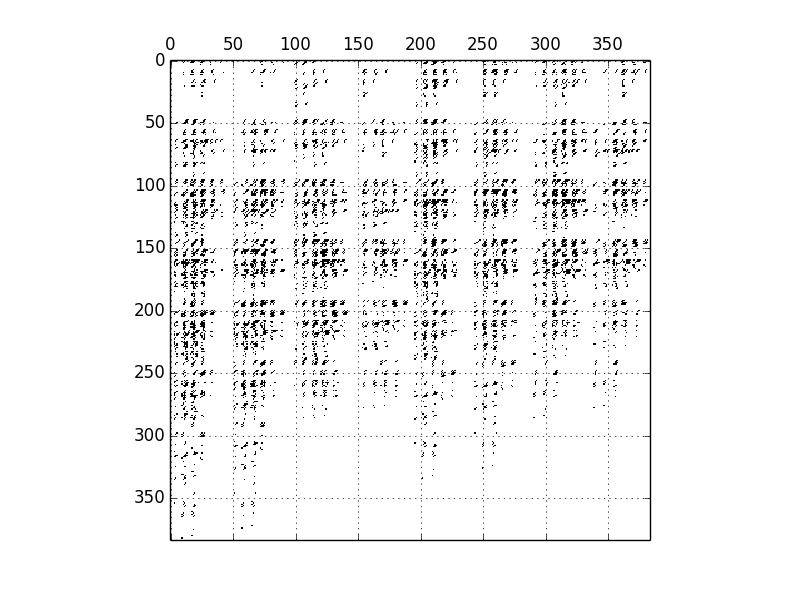
\includegraphics[width=8cm]{B0.png}
\end{center}

Ce système est de multidegré $(3, 2, 2, 2)$, la matrice de Bezout $B(1)$ est de taille $576$. Si on effectue une factorisation QRP sur cette matrice, on sait que les éléments diagonaux seront triés en ordre décroissant, voir figure ci-dessous.
% \begin{center}
% 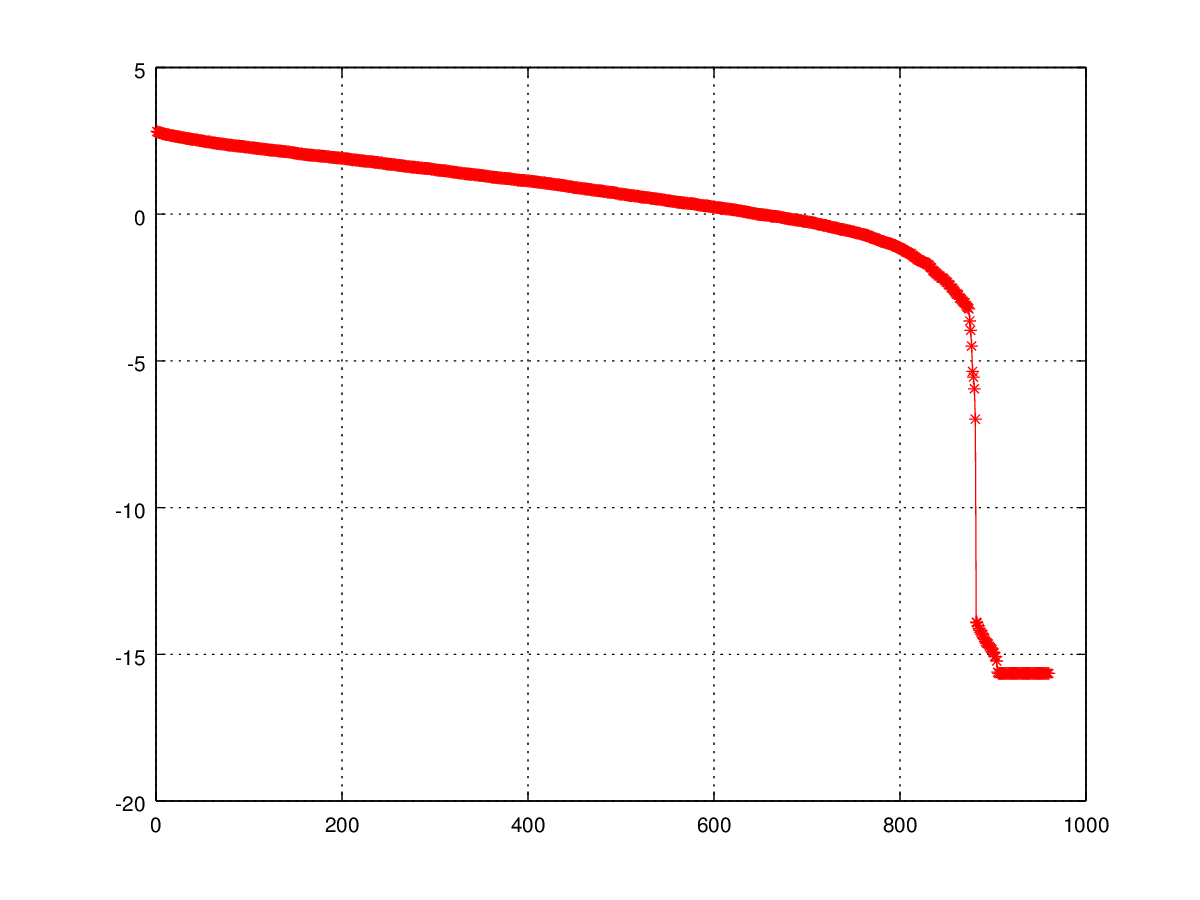
\includegraphics[width=8cm]{qrp.pdf}
% \end{center}
 On s'aperçoit alors que les derniers éléments non nuls décroissent très vite, et qu'il peut devenir difficile de choisir un seuil au dessus duquel les éléments diagonaux seront déclarés "non nuls".
En d'autres termes, le "saut" entre éléments "non-nuls" et éléments proches du epsilon de la machine a tendance à diminuer à mesure que la taille de la matrice augmente, ce qui rend le calcul du rang numérique difficile.\\
Nous pouvons cependant améliorer un peu la situation précédente, en exploitant une propriété de $B(1)$. En effet, en permutant lignes et colones de cette matrice d'une certaine façon, on peut arriver à une structure bloc-triangulaire de $B(1)$.
\begin{center}
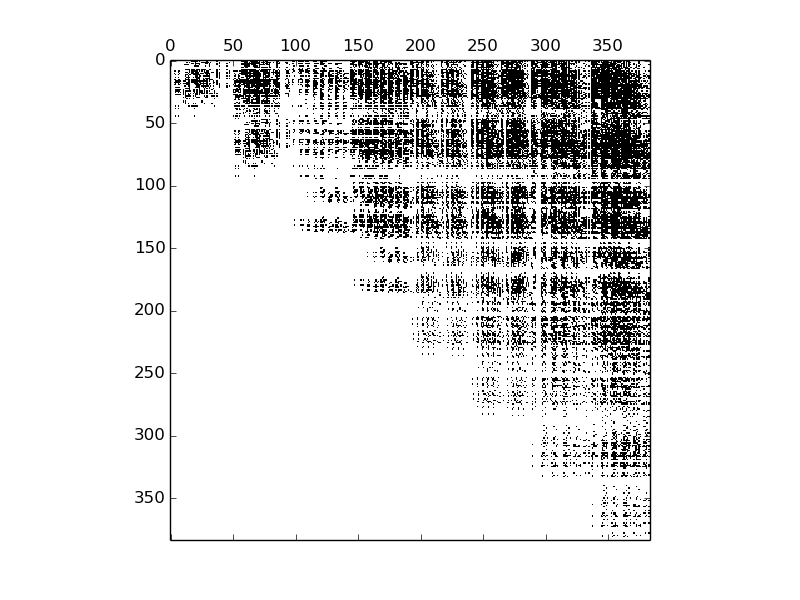
\includegraphics[width=8cm]{B0_tri.png}
\end{center}
En factorisant la matrice bloc après bloc, les éléments diagonaux vont alors décroitre uniquement à l'intérieur de chaque bloc, ce qui permet à la fin de préserver un saut numérique plus grand que dans la première approche. Le graphique ci dessous montre la nouvelle disposition des éléments diagonaux pour le même exemple que précédemment, traité de la deuxième façon.
\begin{center}
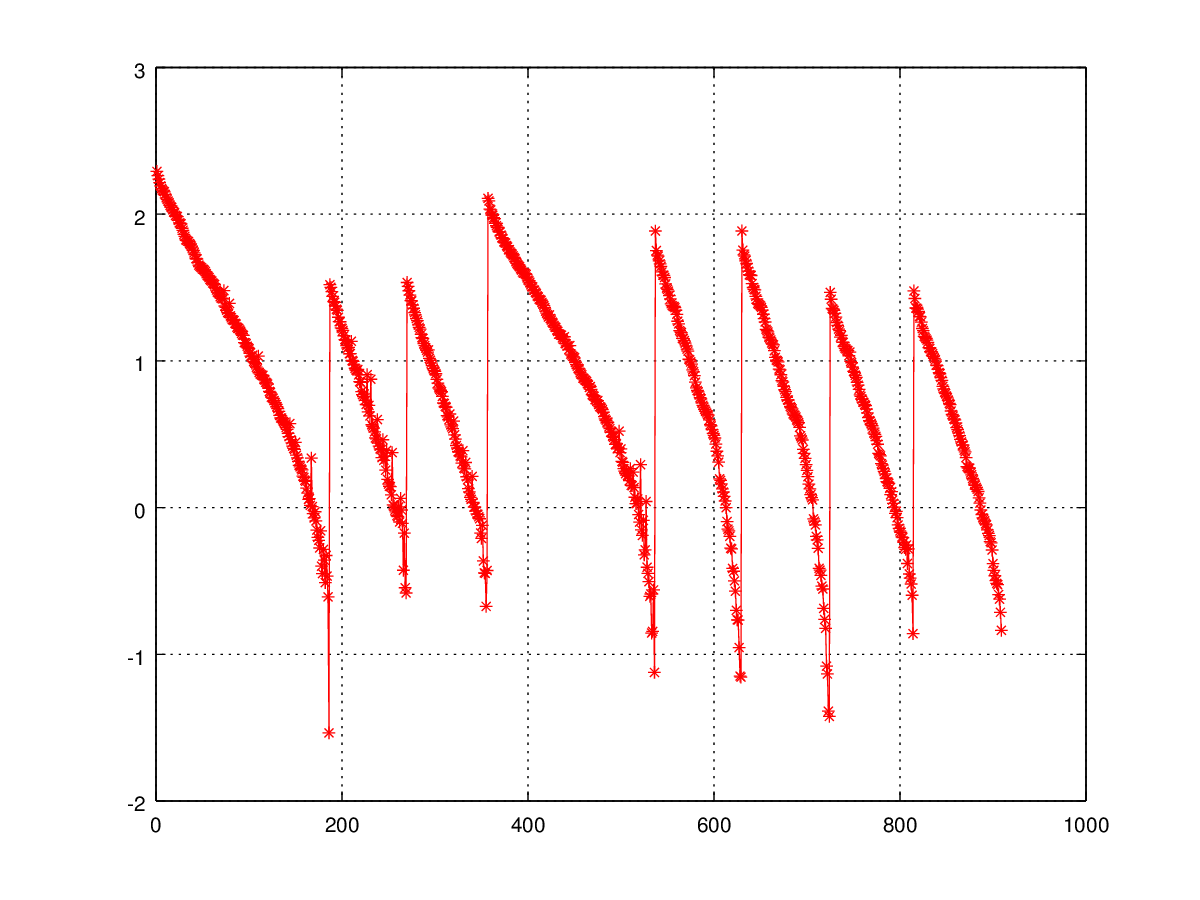
\includegraphics[width=8cm]{bloc_triang.png}
\end{center}
On voit que, malgré une décroissance rapide des éléments diagonaux dans chaque bloc, la plus petite taille de ceux-ci permet au plus petit élément "non-nul" d'être beaucoup plus grand que le epsilon machine, ce qui facilite le calcul du rang numérique.

\section{Expérimentation}
Nous choisissons $n=4$ et le multidegré $deg=[2,2,2,2]$. Le système polynômial s'écrit
\begin{align}
f_1 & =
-x_0^2x_1^2x_2^2 - x_0x_1x_2^2 + x_0x_2^2x_3 - x_1^2x_2 + x_1x_3^2 - x_0^2 + x_1x_2 - x_1 - 1, \nonumber\\
f_2 & =
 -x_1^2x_2^2x_3^2 - x_0^2x_2^2x_3 - x_0x_1x_2x_3^2 + x_0^2x_2 - x_0x_1x_2 + x_1^2x_3 + x_0x_1 - x_1x_2 - 1, \nonumber\\
 f_3 & =
 x_0x_1^2x_2^2x_3^2 + x_0^2x_2^2x_3 - x_0^2x_1x_3^2 + x_0^2x_3^2 - x_0x_1 + 1, \nonumber\\
 f_4 & =
 -x_0^2x_1^2x_2^2x_3^2 - x_0^2x_1x_3^2 - x_0x_2^2x_3^2 - x_1x_2^2 + x_1^2x_3 - x_1^2 - x_1x_3] \nonumber\\
 \end{align}

La matrice de Bezout $B(1)$ est de taille $384$,
 \begin{center}
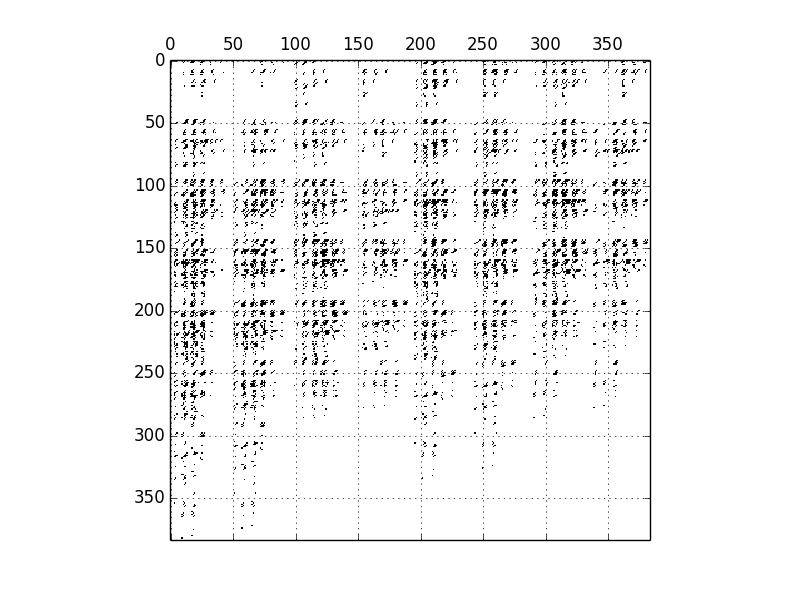
\includegraphics[width=8cm]{B0.png}
\end{center}


En permutant lignes et colonnes on obtient une matrice bloc-triangulaire supérieure
 \begin{center}
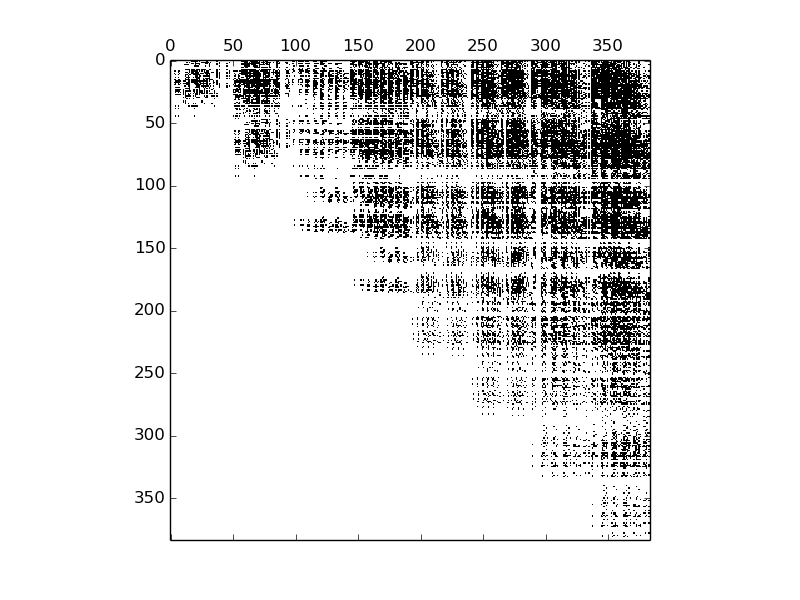
\includegraphics[width=8cm]{B0_tri.png}
\end{center}
dont on peut calculer le noyau facilement. On trouve que rang de $B(1)$ vaut $253$.
Une fois le processus de réduction terminé on obtient des matrices $B(1), B(x_j), j=1,\cdots,n$ de même taille, $B(1)$ étant inversible. On trouve que la dimension de $A$ est $253$. Les matrices compagnon $X_j = B(x_j)B(1)^{-1}$ fournissent alors les racines du système polynômial. Pour chacune des racines obtenues nous vérifions sa qualité en lui appliquant les polynômes $f_i, i=1,\cdots,n$ puis on représente en graphique semi-logarithmique la  valeur absolue du résultat
 \begin{center}
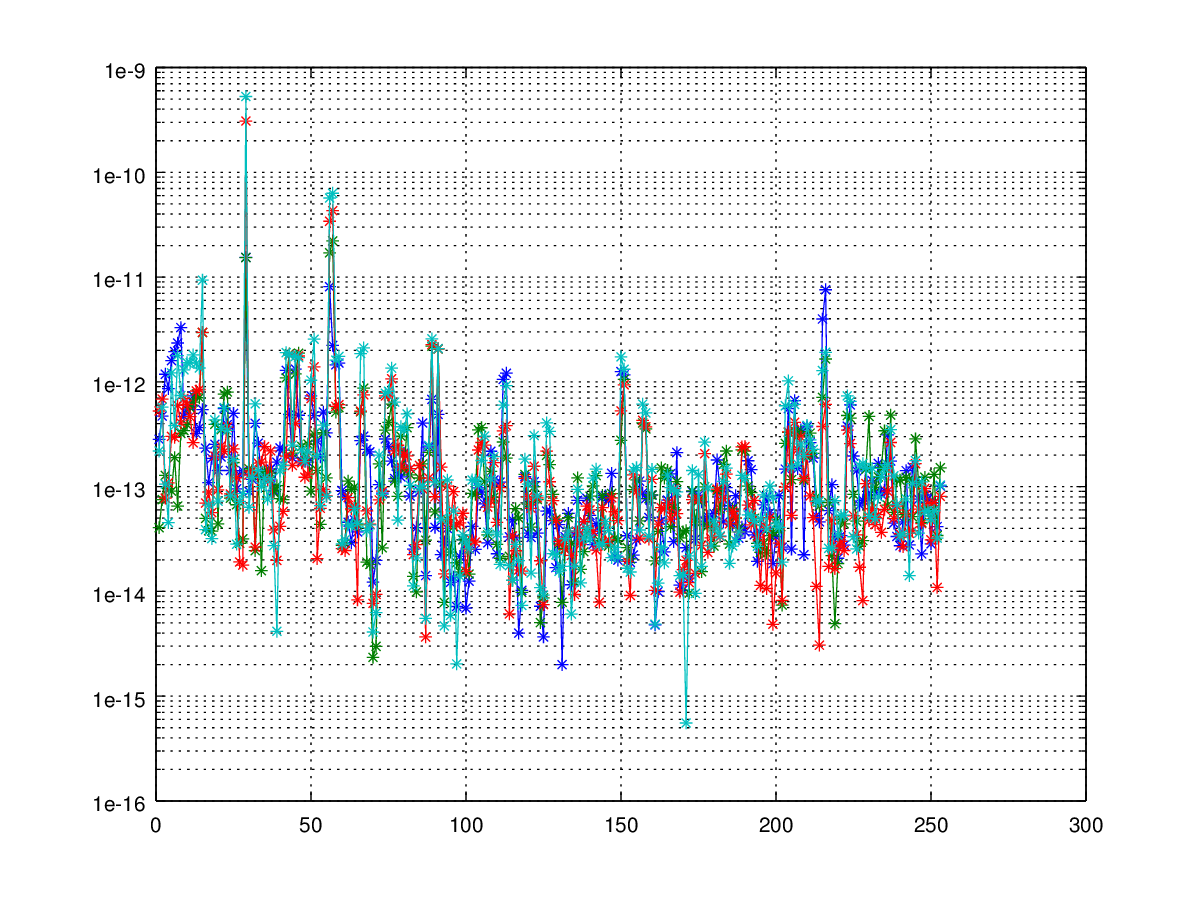
\includegraphics[height=10cm, width=18cm]{f_rac.png}
\end{center}
Les mêmes résultats représentés sous forme d'histogramme
 \begin{center}
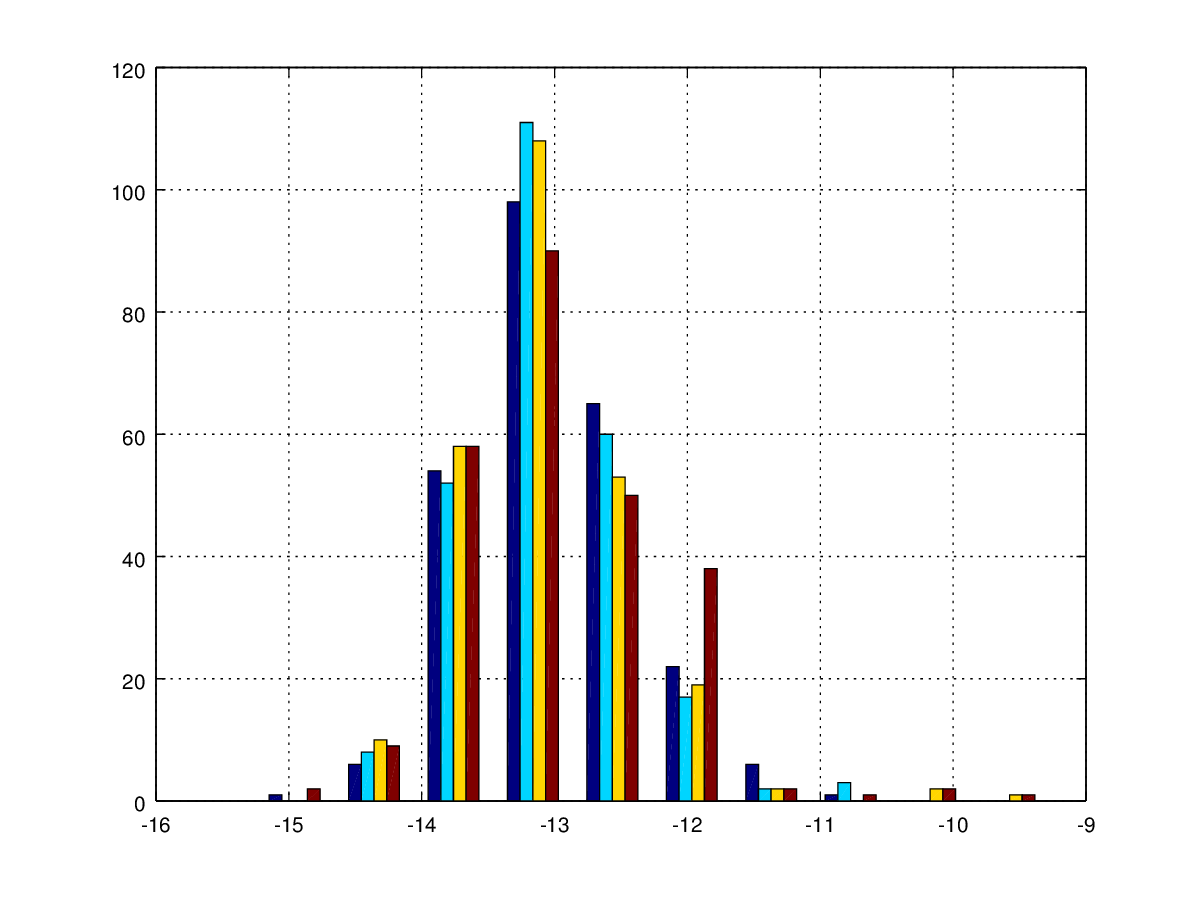
\includegraphics[height=10cm, width=18cm]{f_rac_hist.png}
\end{center}

Dans cet exemple nous voyons que la qualité est excellente pour toutes les racines.
\section{Conclusion et perspectives}
Nous avons proposé une méthode de résolution numérique des systèmes polynômiaux en intersection complète. Cette méthode utilise exclusivement des techniques d'algèbre linéaire numérique. Le principe de la méthode repose sur une conjecture de nature algébrique mais il est facile de tester si les racines obtenues sont numériquement correctes et les racines non satisfaisantes peuvent être écartées.

\begin{thebibliography}{00}

\bibitem{AS}
{Auzinger, Stetter}, {A note }, {SIAM }, {19?}

\bibitem{Barnett}
{S. Barnett}, {A note on the Bezoutian matrix}, {SIAM J. Appl. Math., 22:84-86}, {1972}

\bibitem{Golub}
{G.H. Golub, C.F. van Loan}, {Matrix Computations}, {The Johns Hopkins University Press}, {1989}.

\bibitem{jpc}
{J.P. Cardinal}, {Dualité et algorithmes itératifs pour la résolution de systèmes polynomiaux}, {Thèse présentée devant l'université de Rennes I}, {1993}.

\bibitem{CM}
{J.P. Cardinal, B. Mourrain}, {Algebraic approach of residues and applications}, {in: J. Renegar, M. Shub, S. Smale (Eds.), Proc. AMS-SIAM Summer Seminar on Math. of Numerical Analysis, Park City, Utah, 1995, Lectures in Appl. Math., 32, Amer. Math. Soc, Providence, pp. 189-210}, {1996}

\bibitem{clo}
{D. Cox, J. Little, D. O'Shea}{Ideals, Varieties and Algorithms}
\end{thebibliography}

\end{document}
%%%%%%%%%%%%%%%%%%%%%%%%%%%%%%%%%%%%%%%%%%%%%%%%%%%%%%%%%%%%%%%%%%%%%%%%%%%%%%%%%%%%%%%%%%%%%%%%%%%%%%%%%%%%

$\delta(1) = \sum_{\alpha} x^\alpha \hat{y}_\alpha = \sum_{\beta} \hat{x}_\beta y^\beta$.

Pour fixer les choses nous nous donnons un système de polynômes $f_1, \cdots, f_n$ en $n$ variables, nous appellerons multi-degré de $f$ le $n$-uplet d'entiers $(d_1, \cdots, d_n)$ tel que pour tout $j$, $d_j$ est le maximum des degrés des $f_i$ en la variable $x_j$.\\
Par exemple, si $n = 3$ et
\begin{align}
f_1 & = x_1^2 + x_1x_2^2 - x_1x_2x_3 + 1 \nonumber \\
f_2 & = x_1^2x_2 + x_1 - 5x_2^3 \nonumber \\
f_3 & = x_1x_2^2 + x_3 - 2 \nonumber
\end{align}

\section{Structure triangulaire par blocs et rang de $B(1)$}
Le calcul de la structure de l'algèbre quotient $A =
\C[\bold{x}]/<f>$, effectué au chapitre suivant, nécessitera la
connaissance du rang de la matrice $B(1)$.
\subsection{The singular spectrum of $B_0$ in practice}
\subsection{Using the hidden block-triangular structure of $B_0$ to improve its rank determination}

Multiplions les premières colonnes de $B_0$ et $B_1$ à gauche par $\bold{x}^T$ pour obtenir des polynômes en $x$

Nous constatons que, modulo $<f(x)>$, on a la relation $x\bold{x}^TB_0(:, 1) = \bold{x}^TB_1(:, 1)$ et que cette propriété est vraie pour toutes les colonnes de $B_0$ et $B_1$.
En d'autres termes, toute colonne de $B_0$, vue comme un élément de $A_x$, multipliée par $x$, est égale à la colonne de même indice de $B_1$
Synthétiquement nous avons les relations dans $A_x^d$ et $A_y^d$:
\begin{equation}
\begin{array}{c}
\bold{x}^TB_0x = \bold{x}^TB_1\\
yB_0\bold{y} = B_1\bold{y}
\end{array}
\end{equation}

Soit $\{x^\alpha y^\beta, (\alpha, \beta) \in A\times B\}$ l'ensemble des monômes apparaissant dans les polynômes de Bezout $\delta(x_j), j = 0,\cdots ,n$.
Pour chaque $j$ écrivons $\delta(x_j) = \sum_{\alpha\in A} x^\alpha \hat{y}_j^\alpha = \sum_{\beta\in B} \hat{x}_j^\beta y^\beta$.
Ecrivons le polynôme de Bezout $\delta(1) = \sum_{\alpha,\beta} b_{\alpha\beta} x^\alpha y^\beta$ comme une somme de monômes.
Pour chaque $\alpha$ posons $\hat{y}_\alpha = \sum_{\beta} b_{\alpha\beta} y^\beta$
et pour chaque $\beta$ posons $\hat{x}_\beta = \sum_{\alpha} b_{\alpha\beta} x^\alpha$, de sorte que

		\hat{\bold{y}} & = & B_0\bold{y}^T \\
		\hat{\bold{y}}_j & = & B_j\bold{y}^T, \quad j=1\cdots n
\{\hat{y}_\alpha\} & =  \{ -y1y_2 + y_1^3, -y_1 - y_1^2y_2, 0, y_1^2, -y_1y_2, -y_1 \}  \nonumber \\
 \{\hat{x}_\beta\} & = \{0, -x_2 - x_1x_2^2, -1 - x_1x_2, x_1, -x_2, 1 \}  \nonumber \\
 \{y^\beta\} & =  \{1, y_1, y_1y_2, y_1^2, y_1^2y_2, y_1^3 \}  \nonumber

Reécrivons maintenant toutes les colonnes de nos deux matrices en tenant compte de la relation $x^2 = -2 + 3x$. Les colonnes de $B(x^3)$ se reécrivent alors $4 - 6x$ pour la première, $-6 + 7x$ pour la deuxième et $0$ pour la troisième. La matrice $B(1)$ quand à elle, est inchangée ce qui donne
$$
\begin{array}{c|ccc}
B(1) & 1 & y & y^2\\
\hline
1 & -3 & 1 & 0\\
x & 1 & 0 & 0\\
x^2 & 0 & 0 & 0
\end{array}
\hspace{1cm}
\begin{array}{c|ccc}
B(x^3) & 1 & y & y^2\\
\hline
1 & 4 & -6 & 0\\
x & -6 & 7 & 0\\
x^2 & 0 & 0 & 0
\end{array}
$$
matrices que nous pouvons maintenant écrire dans le système d'indices $\bold{x} = (1, x)$ et $\bold{y} = (1, y)$
\begin{equation}
\label{B1x3}
\begin{array}{c|cc}
B(1) & 1 & y \\
\hline
1 & -3 & 1 \\
x & 1 & 0
\end{array}
\hspace{1cm}
\begin{array}{c|cc}
B(x^3) & 1 & y \\
\hline
1 & 4 & -6 \\
x & -6 & 7 \\
\end{array}
\end{equation}
